% HW2 high dimensional data

\documentclass[12pt, leqno]{article}
\usepackage{amsfonts, amsmath, amssymb}
\usepackage{amsthm}
\usepackage{mathtools}
\usepackage{fancyhdr}
\usepackage{hyperref}
\usepackage{graphicx}
\usepackage{caption}
\usepackage{subcaption}
\usepackage{float}
\usepackage{mathrsfs}
\usepackage{array} 
\usepackage{rotating}
%\usepackage{babel}
\providecommand{\abs}[1]{\lvert#1\rvert}
\providecommand{\norm}[1]{\lVert#1\rVert}
\newcommand{\macheps}{\epsilon_{\mbox{\scriptsize mach}}}
\let\oldhat\hat
\renewcommand{\vec}[1]{\mathbf{#1}}
\renewcommand{\hat}[1]{\oldhat{{#1}}}
\def\rp{\ensuremath \mathbb{R}^p}
\def\rpp{\ensuremath \mathbb{R}^{p \times p}}
\def\s{\ensuremath\Sigma}
\def\om{\ensuremath\Omega}
\def\pd{\ensuremath\mathbb{P}^+}
\def\pg{\ensuremath\mathbb{P}_{{G}}}
\def\E{\ensuremath\mathbb{E}}
\def\normdist[#1]#2{\ensuremath \sim \mathcal{N} (#1,#2) }
\def\ndist1{\ensuremath \sim \mathcal{N}  (\mu, \sigma)}
\def\ndistvec{\ensuremath \sim \mathcal{N}_p ( {\mu},  {\Sigma})}
\def\lra{\ensuremath\Leftrightarrow}
\def\stackrel#1#2{\mathrel{\mathop{#2}\limits^{#1}}}
\newcommand\ind{\protect\mathpalette{\protect\independenT}{\perp}}
\def\independenT#1#2{\mathrel{\rlap{$#1#2$}\mkern2mu{#1#2}}}
\makeatletter
\newtheorem{thm}{Theorem}[]
\newtheorem{lemma}{Lemma}[]
\newtheorem{defn}[thm]{Definition}
\newcommand{\sign}{\mathrm{sign}}
\newcommand{\distas}[1]{\mathbin{\overset{#1}{\kern\z@\sim}}}%
\newsavebox{\mybox}\newsavebox{\mysim}
\newcommand{\dist}[1]{%
  \savebox{\mybox}{\hbox{\kern3pt$\scriptstyle#1$\kern3pt}}%
  \savebox{\mysim}{\hbox{$\sim$}}%
  \mathbin{\overset{#1}{\kern\z@\resizebox{\wd\mybox}{\ht\mysim}{$\sim$}}}%
}
\makeatother

\begin{document}
\pagestyle{fancy}
\lhead{TA,RB,SR,AS}
\rhead{STA7934}

\begin{center}
{\large {\bf Homework 2 - Analysis of High Dimensional Data}} \\
{\it{Tavis Abrahamsen, Ray Bai, Syed Rahman and Andrey Skripnikov}} \\
\end{center}

\paragraph{Logistic Regression with Lasso Penalty} Consider a classification problem, where the response is
binary $y \in \{0,1\}$ and the predictor variables numerical. .Generate a design matrix $X$ of size 5,000 by 300 (i.e. 5,000 observations and 300 variables). Generate the corresponding response $y$ by selecting an appropriate coefficient vector $\beta$ and adding a noise term.

Consider a model where the true coefficent vector has only 20 non-zero
elements and another with 75 non-zero elemensts. Devise a sub-gradient
based algorithm (soft-thresholding) to solve the problem, where the Gram matrix $X'X$ is well-conditioned.

Compare the performance of your algorithm for a grid of the tuning parameter $\lambda$.

\paragraph{} We are interested in solving the
logistic regression from last time with a $lasso$ penatly added
on. Recall that last time our objective is to minimize the negative log likelihood 
\[
-l(\beta) = -\sum_{i=1}^{n} [y_i \log (\pi_i)+ (1-y_i) \log (1-\pi_i)]
\]
where 
\[
\log (\frac{\pi_i}{1-\pi_i}) = {x_i' \beta}.
\]
While $\nabla (-l(\beta)) = 0$ has no closed form solutions, it is a convex function as we
showed last time and hence we can use the gradient descent algorithm 
\[
\beta^{k+1} = \beta^{k} - \alpha^k \nabla (-l(\beta^k))
\]
where $\alpha^k$ is a suitably chosen stepsize and $-\nabla l(\beta^k) = -X'(y-\frac{e^{X \beta}}{1+e^{X
    \beta}})$.
This time we have an added constaint. The primal problem we are
interested in solving can be formulated as:
\begin{align*}
\textbf{PRIMAL:}&
\arg\min_{\beta \in \mathbb{R}^p} -l(\beta) \\
&\text{subject to } \norm{\beta}_1 \leq t
\end{align*}
which is a convex problem. Hence we can invoke Slater's condition as
$\exists \text{ a strictly feasible } \beta$. Hence there is no duality
gap and we can instead solve the dual problem:
\begin{align*}
\textbf{DUAL:}&
\arg\max g(\lambda) = \arg\max \inf_{\beta \in \mathbb{R}^p}(-l(\beta)+\lambda(\norm{\beta}_1-t)) \\
&\text{subject to } \lambda \geq 0
\end{align*}
As $g(\lambda)$ is not differentiable, we have to use
subdifferentials. For $\beta$ to satisfy $\inf_{\beta \in
  \mathbb{R}^p}(-l(\beta)+\lambda(\norm{\beta}_1-t))$, we must have
that $\nabla l(\beta) = \lambda \sign(\beta)$, where 
\[
(\sign(\beta))_i = \sign(\beta_i)  = \begin{cases} +1 \text { if }
  \beta_i>0 \\
0 \text { if }
  \beta_i=0 \\
-1 \text { if }
  \beta_i<0
\end{cases}
\] 


This is because a subgradient of
$-l(\beta)+\lambda(\norm{\beta}_1-t)$ is $-\nabla l(\beta)+ \lambda
\sign({\beta})$. Also note that $\nabla l(\beta) = \lambda \sign(\beta)$ is independent of $t$. This suggests that we
can solve the dual problem ignoring $t$ altogether and use the following subgradient descent scheme:
\begin{align*}
\beta^{k+1} &= \beta^{k} - \alpha^k( -\nabla l(\beta^k)+ \lambda
\sign({\beta^k})) \\
&= \beta^{k} - \alpha^k( -X'(y-\frac{e^{X \beta^k}}{1+e^{X
    \beta^k}})+ \lambda
\sign({\beta^k})) 
\end{align*}
and 
\begin{align*}
\beta_{est}^{k+1} 
= \arg\min_{i = 1,...,k+1}
  (-l(\beta^i)+\lambda(\norm{\beta^i}_1).
\end{align*}
One important difference is that the choice of stepsize has to be
prespecified. Due to the superior asymptotic properties, we choose
diminishing stepsizes $\alpha^k = \frac{1}{k}$ such that $\sum_{i=1}^k (\alpha^k)^2 < \infty$
and $\sum_{i=1}^k \alpha^k = \infty$. 
\paragraph{} In generating our data we essentially used the methods
from last time to generate a design matrix $X \in \mathbb{R}^{5000
  \times 300}$ such that $X'X$ has
condition number, $CN(X) = 1$. We can do this by generating a random matrix,$A \in \mathbb{R}^{5000
  \times 300}$, and
doing an SVD to get $A = U \Sigma V'$, where $U \in \mathbb{R}^{5000
  \times 5000}$ and $V \in \mathbb{R}^{300
  \times 300}$ are
orthonormal matrices of the right dimensions. Then let
\[X \coloneqq
U \begin{pmatrix} I \\ 0 \end{pmatrix} V' = U \begin{pmatrix} V' \\
  0 \end{pmatrix}. \] Thus $CN(X) = CN(U) CN(V) = 1$ and generate 
$\beta_1 \distas{} \mathcal{N}_d(0,2I_{d \times d})$ with $d = 20 \text{
  or }75
$ being the number of non-zero elements. Now let
\[
\beta = \begin{pmatrix} \beta_1 \\
0_{(p-d) \times 1}
\end{pmatrix}
\] and 
\[
\pi_i = \frac{e^{x_i' \beta}}{1+e^{x_i' \beta}}, \quad i = 1,...,n.
\] Then generate $y_i
\distas{ind} Bin(1,\pi_i)$. The value of $\lambda$'s used where from 0.1
through to 1.5 incremented by 0.1 at each step. While there is no good
stopping criteria, the one we used was $\text{Epsilon or } \epsilon < 10^{-5}$
where  
\[
\epsilon \coloneqq \norm{\beta_{est} -
  \beta_{k}}_2.
\] 
and the maximum number of iterations was set to 10,000. Unfortunately,
the stopping criteria was almost never reached, and the program
usually ran for the maximum number of iterations.

We chose as optimal $\lambda$ to the smallest $\lambda$ at which the
negative log-likelihood, sparsity and shrinkage and the norm of
$\beta_{est} - \beta_{true}$ began to taper off. These results
are presented below. When the number of non-zero elements in
$\beta_{true}$ was 20, the optimal $\lambda$ was around 0.7.  This is 
when $\beta_{est}$ gets very close to its highest value in terms of out measure
of sparseness and shrinkage as can be seen in Figure
\ref{fig:sparse}. Additionally, as Figure \ref{fig:20} shows the norm
of the estimated beta from the true beta is slightly below 7.5. The negative log likelihood plus the
penalty term reaches slightly around 3,470. While a higher value of
$\lambda$ seems to lead to marginally higher values ot this term, we
are more interested in getting sparse solutions.  When $\lambda$ was
very small $(\leq 0.2)$, the program did terminate after a few
thousand iterations. However, as mentioned before, in most cases, the
program ran for $10,000$ iterations. 

When the number of non-zero elements in $\beta_{true}$ was 75, the
program never seemed to reach the stopping criteria and reached the
maximum number of iterations allowed at 10,000 for all $\lambda$. Increasing the maximum
number of iterations to 100,000 didn't seem to make a difference in
this regard either. The best results were still at $\lambda = 1.0$,
with the normed difference between the estimated beta from the true
beta reaching almost as low as 15, as can be
seen in Figure \ref{fig:75}. As in the case of $20$ non-zero elements
in $\beta_{true}$, Figure \ref{fig:sparse}
shows, our measure of sparsity and shrinkage keeps on increasing
towards 300. In this case, the negative log likelihood plus the
penalty term reaches slightly below 3,460 and from thereon out keeps
increasing at a very
low rate as the value to $\lambda$ keeps increasing.

\begin{figure}
\centering 
\begin{subfigure}[b]{0.5\textwidth}
  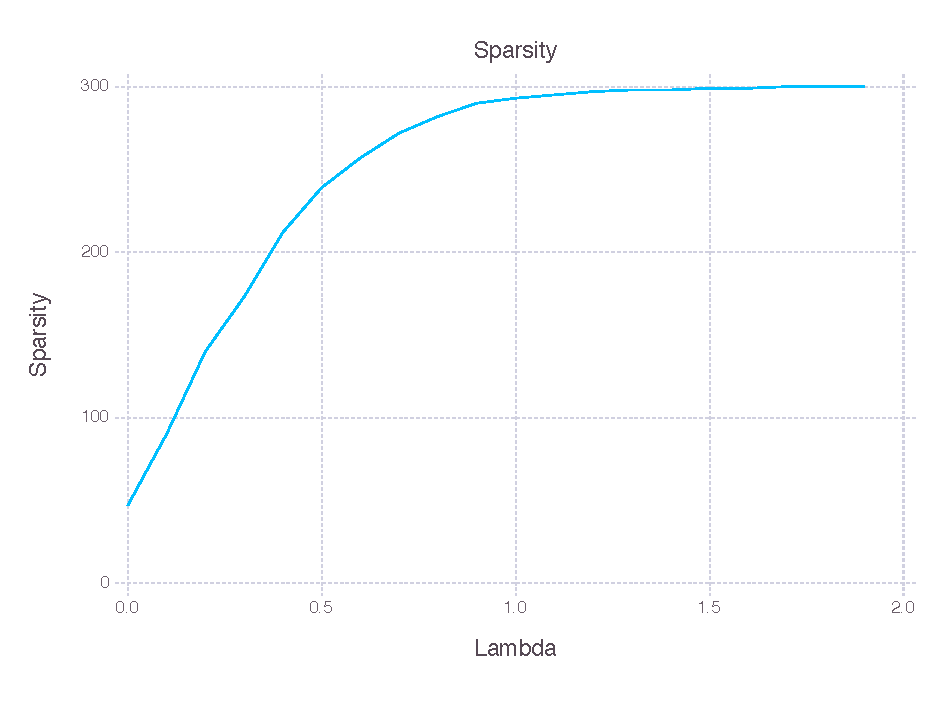
\includegraphics[width=\textwidth]{sparsityplotcount-20.pdf}
  \caption{A plot of the sparsity/shrinkage versus $\lambda$. The criteria for
    sparsity/shrinkage was the number of elements of $\beta_{est}$
    smaller than $10^{-3}$ when $\beta_{true}$ had 20 non-zero elements}
\label{sparse20}
\end{subfigure}\\
\begin{subfigure}[b]{0.5\textwidth}
  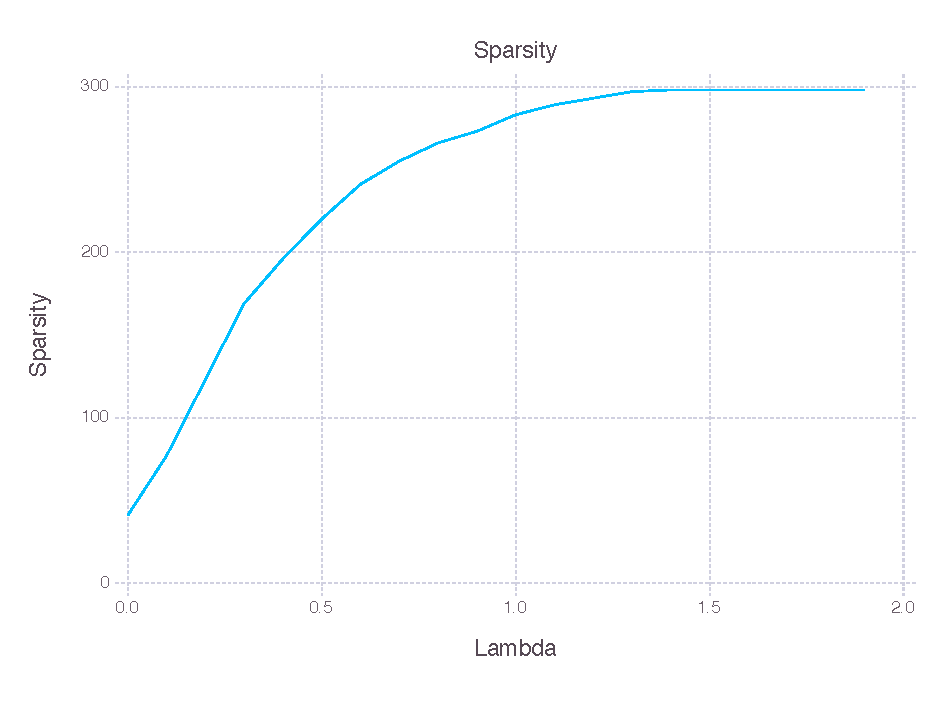
\includegraphics [width=\textwidth]{sparsityplotcount-75.pdf}
  \caption{A plot of the sparsity/shrinkage versus $\lambda$. The criteria for
    sparsity/shrinkage was the number of elements of $\beta_{est}$
    smaller than $10^{-3}$ when $\beta_{true}$ had 75 non-zero elements}
\label{sparse75}
\end{subfigure}
        \caption{A plot of the sparsity/shrinkage versus $\lambda$. }\label{fig:sparse}
\end{figure}

\begin{figure}
\centering 
\begin{subfigure}[b]{0.5\textwidth}
                \includegraphics[width=\textwidth]{{errorcplot11-20.pdf}}
                \caption{Epsilon for $\lambda = 1.1$}
                \label{fig:errorc20}
        \end{subfigure}\\
\begin{subfigure}[b]{0.5\textwidth}
                \includegraphics[width=\textwidth]{{trueerrorplot11-20.pdf}}
                \caption{Norm of $\beta_{true} - \beta_{est}$ when $\lambda = 1.1$}
                \label{fig:true20}
        \end{subfigure}
        \caption{Error plots for Subgradient Descent Algorithm with
          $\beta_{true}$ having 20 non-zero elements and $\lambda = 1.1$.}\label{fig:20}
\end{figure}

\begin{figure}
\centering 
\begin{subfigure}[b]{0.5\textwidth}
                \includegraphics[width=\textwidth]{{errorcplot10-75.pdf}}
                \caption{Epsilon for $\lambda = 1.0$}
                \label{fig:errorc20}
        \end{subfigure}\\
\begin{subfigure}[b]{0.5\textwidth}
                \includegraphics[width=\textwidth]{{trueerrorplot10-75.pdf}}
                \caption{Norm of $\beta_{true} - \beta_{est}$ when $\lambda = 1.0$}
                \label{fig:true20}
        \end{subfigure}
        \caption{Error plots for Subgradient Descent Algorithm with
          $\beta_{true}$ having 75 non-zero elements and $\lambda = 1.0$.}\label{fig:75}
\end{figure}

\pagebreak 

\paragraph{Appendix}

\begin{verbatim}
#Pkg.add("Distributions")
#Pkg.add("PyPlot")
#Pkg.add("Gadfly")
#Pkg.add("Cairo")

using PyPlot
using Distributions
using Gadfly


srand(12345)
print("enter p "); p = int(readline(STDIN))
print("enter n  "); n = int(readline(STDIN))
print("enter notsparse  "); notsparse = int(readline(STDIN))

function gradf(X::Matrix{Float64},y::Vector{Int}, 
p::Vector{Float64}, lambda::Float64,beta::Vector{Float64})
    -X'*(y-p)+lambda*sign(beta)
end

function neglogLkhd(probOld::Vector{Float64}, 
y::Vector{Int}, lambda::Float64, betaOld::Vector{Float64})
    n = length(y)
    z = zeros(n)
    p = length(betaOld)
    penaltyterm = zeros(p)
    for i = 1:n
            term1 = y[i]*log(probOld[i])
            term2 = (1-y[i])*log(1-probOld[i])
            z[i] = -term1-term2
        end
    	for i = 1:p
            penaltyterm[i] = lambda*abs(betaOld[i])
        end    
	(sum(z) + sum(penaltyterm))
end

expit(x::Float64) = exp(x)/(1+exp(x))
expit(V::Vector{Float64}) = [expit(v) for v in V]

rbern(p::Float64) = 0<p<1?rand(Bernoulli(p))
:error("p not in (0,1)")
rbern(V::Vector{Float64}) = [rbern(v) for v in V]

dataMat = rand(n,p)
(U,S,V) = svd(dataMat); @elapsed svd(dataMat)
#d = rand(Uniform(0,sqrt(30)),p)
#X = U*diagm(d)*V'
X = U*V'
betaTrue = rand(Normal(0,2),notsparse)
betaTrue =  [betaTrue;zeros((p-notsparse))]
Xbeta = X*betaTrue
probTrue = expit(Xbeta)
y = rbern(probTrue)

maxcount = 15
sparsityvec = zeros(maxcount)
for count = 1:maxcount
lambda = 0.1*count 
maxIter = 100000
betaOld = zeros(p)+1
Xbeta = X*betaOld
probOld = expit(Xbeta)
alpha = 1
tol = 10.0^-5
iter = 0
eps = 1
betamat = betaOld 
betaopt = betaOld
Xbeta = X*betaOld
probopt = expit(Xbeta)

neglogLkhdvec = neglogLkhd(probopt,y,lambda,betaopt)
epsvec = eps
trueerror = sqrt(dot(betaopt-betaTrue,betaopt-betaTrue))
trueerrorvec = trueerror

while iter< maxIter && eps > tol
	betaNew = betaOld - (alpha/(iter+1))*gradf(X,y,
probOld,lambda, betaOld)
	Xbeta = X*betaNew
    	probNew = expit(Xbeta)
    	eps = sqrt(dot(betaNew-betaopt,betaNew-betaopt))
	trueerror = sqrt(dot(betaopt-betaTrue,betaopt-betaTrue))

	if neglogLkhd(probNew,y,lambda,betaNew)
<neglogLkhd(probopt,y,lambda,betaopt)
           betaopt = betaNew
           Xbeta = X*betaopt
           probopt = expit(Xbeta)
        end

	betaOld = betaNew
	probOld = probNew

	if (iter%100) == 0
	   println("Iteration:",iter," " ,
neglogLkhd(probOld,y,lambda,betaOld)," ",eps,"\n")
	end
	   
	neglogLkhdvec = [neglogLkhdvec 
neglogLkhd(probopt,y,lambda,betaopt)]
	epsvec = [epsvec eps]
	trueerrorvec = [trueerrorvec trueerror]
	iter = iter+1
end
end

\end{verbatim}

\begin{figure}
        \centering
        \begin{subfigure}[b]{0.4\textwidth}
                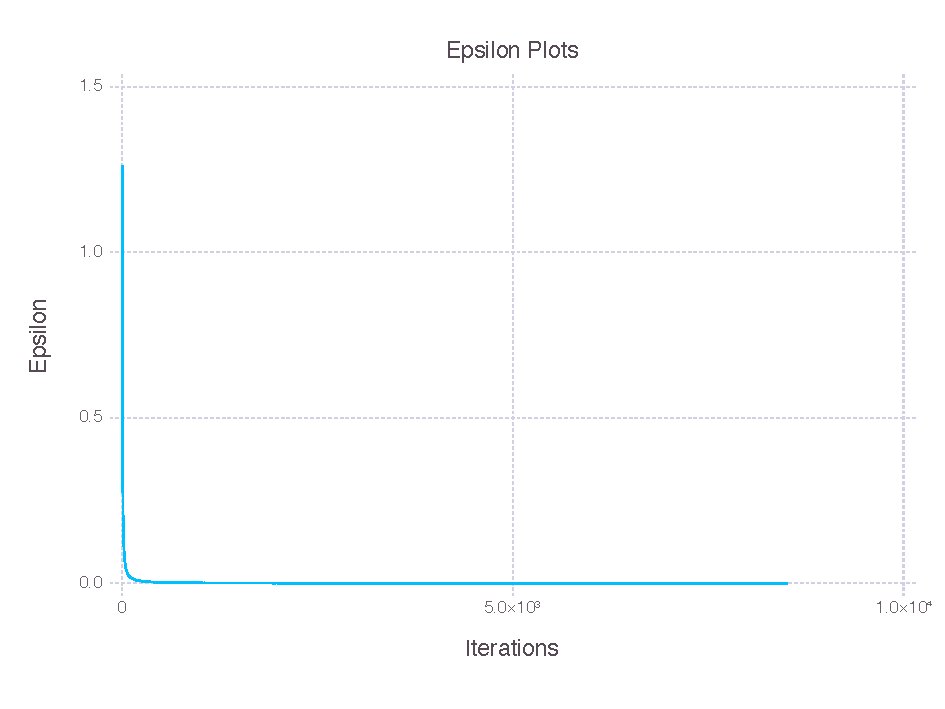
\includegraphics[width=\textwidth]{errorcplot1-20.pdf}
                \caption{$\lambda = 0.1$}
                \label{}
        \end{subfigure}
        \begin{subfigure}[b]{0.4\textwidth}
                \includegraphics[width=\textwidth]{{errorcplot2-20.pdf}}
                \caption{$\lambda = 0.2$}
                \label{}
        \end{subfigure}
        \begin{subfigure}[b]{0.4\textwidth}
                \includegraphics[width=\textwidth]{{errorcplot3-20.pdf}}
                \caption{$\lambda = 0.3$}
                \label{}
        \end{subfigure}
        \begin{subfigure}[b]{0.4\textwidth}
                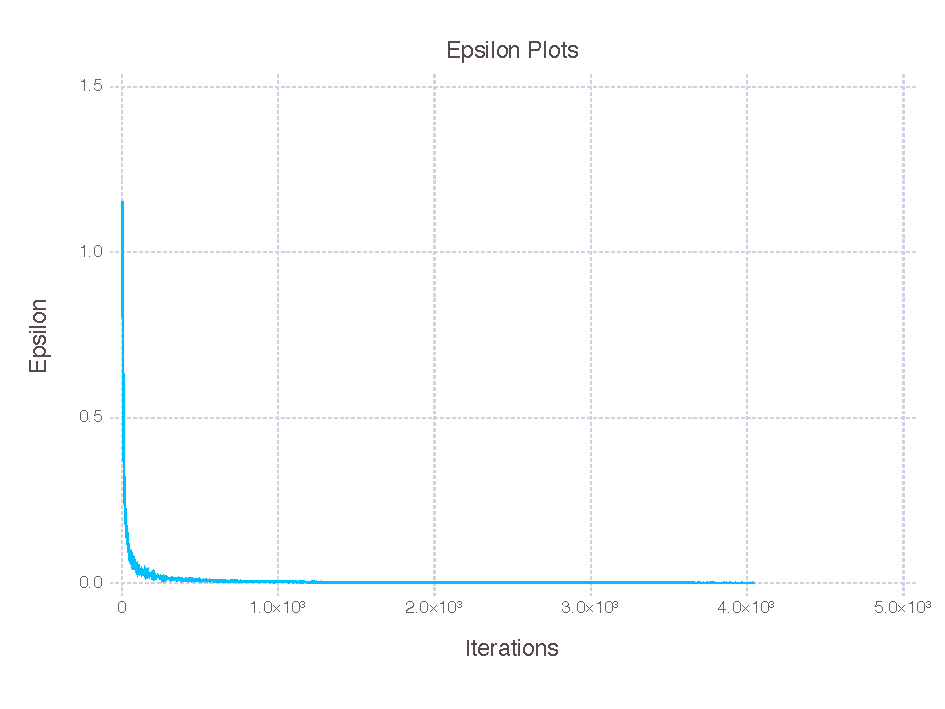
\includegraphics[width=\textwidth]{errorcplot4-20.pdf}
                \caption{$\lambda = 0.4$}
                \label{}
        \end{subfigure}%
        \begin{subfigure}[b]{0.4\textwidth}
                \includegraphics[width=\textwidth]{{errorcplot5-20.pdf}}
                \caption{$\lambda = 0.5$}
                \label{}
        \end{subfigure}
        \caption{A plot of the Epsilon at each
          iteration with 20 non-sparse entries}\label{fig:errorcs20-1}
\end{figure}
\begin{figure}
        \centering
        \begin{subfigure}[b]{0.4\textwidth}
                \includegraphics[width=\textwidth]{{errorcplot6-20.pdf}}
                \caption{$\lambda = 0.6$}
                \label{}
        \end{subfigure}
        \begin{subfigure}[b]{0.4\textwidth}
                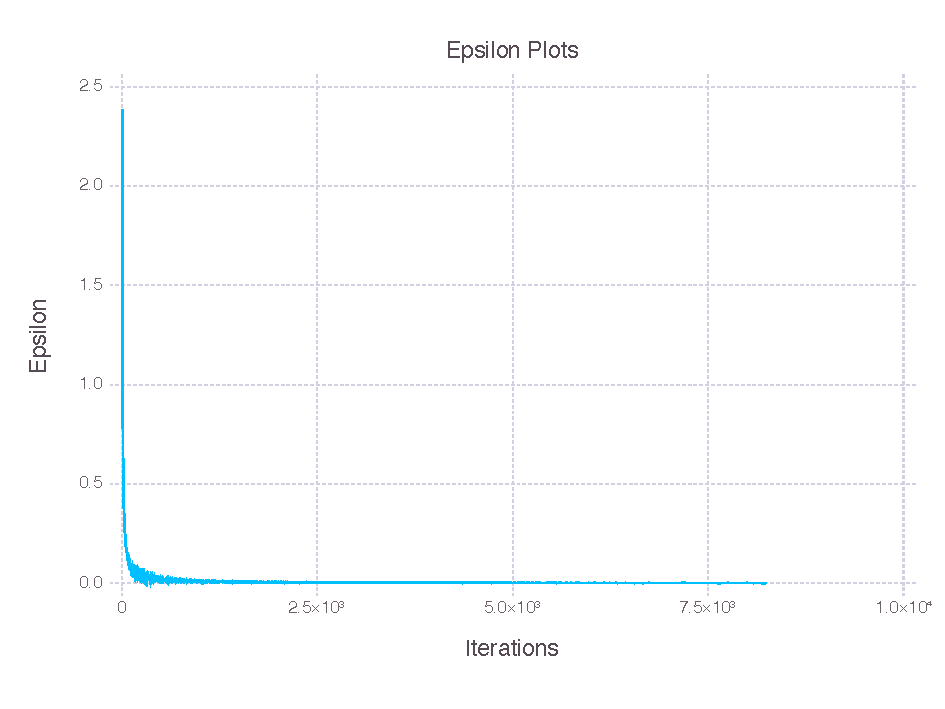
\includegraphics[width=\textwidth]{errorcplot7-20.pdf}
                \caption{$\lambda = 0.7$}
                \label{}
        \end{subfigure}
        \begin{subfigure}[b]{0.4\textwidth}
                \includegraphics[width=\textwidth]{{errorcplot8-20.pdf}}
                \caption{$\lambda = 0.8$}
                \label{}
        \end{subfigure}
        \begin{subfigure}[b]{0.4\textwidth}
                \includegraphics[width=\textwidth]{{errorcplot9-20.pdf}}
                \caption{$\lambda = 0.9$}
                \label{}
        \end{subfigure}
        \begin{subfigure}[b]{0.4\textwidth}
                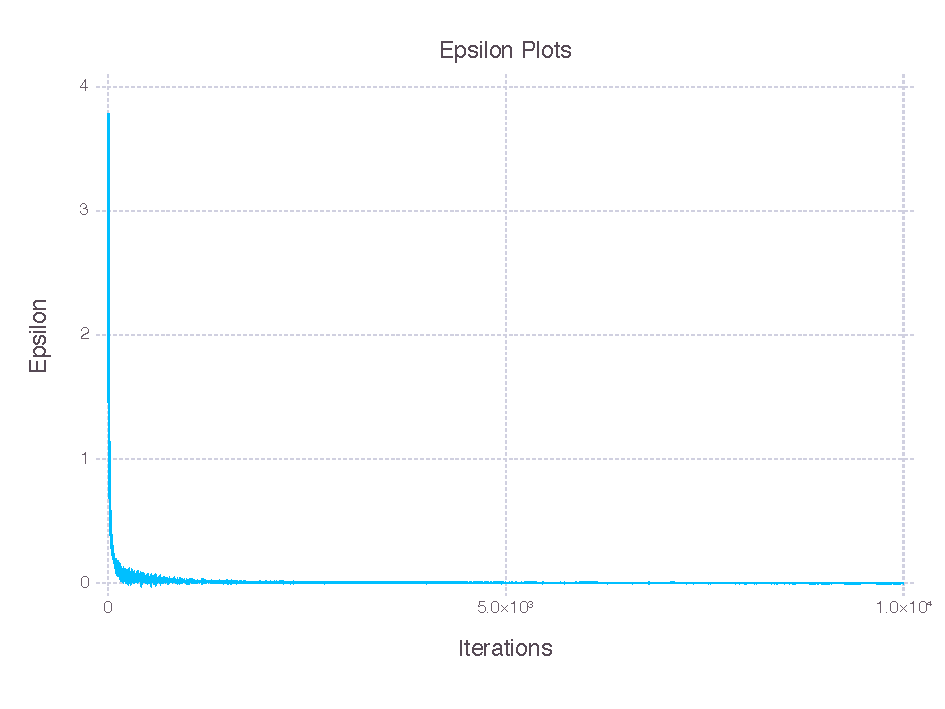
\includegraphics[width=\textwidth]{errorcplot10-20.pdf}
                \caption{$\lambda = 1.0$}
                \label{}
        \end{subfigure}%
        \caption{A plot of the Epsilon at each
          iteration with 20 non-sparse entries}\label{fig:errorcs20-2}
\end{figure}
\begin{figure}
        \centering
        \begin{subfigure}[b]{0.4\textwidth}
                \includegraphics[width=\textwidth]{{errorcplot11-20.pdf}}
                \caption{$\lambda = 1.1$}
                \label{}
        \end{subfigure}
        \begin{subfigure}[b]{0.4\textwidth}
                \includegraphics[width=\textwidth]{{errorcplot12-20.pdf}}
                \caption{$\lambda = 1.2$}
                \label{}
        \end{subfigure}
        \centering
        \begin{subfigure}[b]{0.4\textwidth}
                \includegraphics[width=\textwidth]{{errorcplot13-20.pdf}}
                \caption{$\lambda = 1.3$}
                \label{}
        \end{subfigure}
        \begin{subfigure}[b]{0.4\textwidth}
                \includegraphics[width=\textwidth]{{errorcplot14-20.pdf}}
                \caption{$\lambda = 1.4$}
                \label{}
        \end{subfigure}
        \centering
        \begin{subfigure}[b]{0.4\textwidth}
                \includegraphics[width=\textwidth]{{errorcplot15-20.pdf}}
                \caption{$\lambda = 1.5$}
                \label{}
        \end{subfigure}
        \caption{A plot of the Epsilon at each
          iteration with 20 non-sparse entries}\label{fig:errorcs20-3}
\end{figure}
\begin{figure}
        \centering
        \begin{subfigure}[b]{0.4\textwidth}
                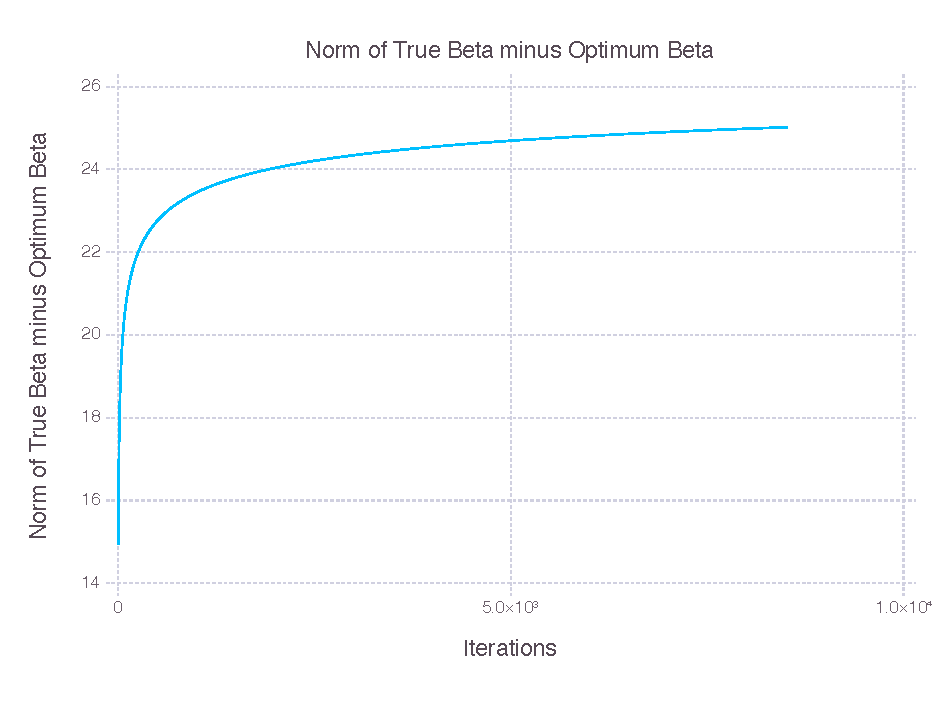
\includegraphics[width=\textwidth]{trueerrorplot1-20.pdf}
                \caption{$\lambda = 0.1$}
                \label{}
        \end{subfigure}
        \begin{subfigure}[b]{0.4\textwidth}
                \includegraphics[width=\textwidth]{{trueerrorplot2-20.pdf}}
                \caption{$\lambda = 0.2$}
                \label{}
        \end{subfigure}
        \begin{subfigure}[b]{0.4\textwidth}
                \includegraphics[width=\textwidth]{{trueerrorplot3-20.pdf}}
                \caption{$\lambda = 0.3$}
                \label{}
        \end{subfigure}
        \begin{subfigure}[b]{0.4\textwidth}
                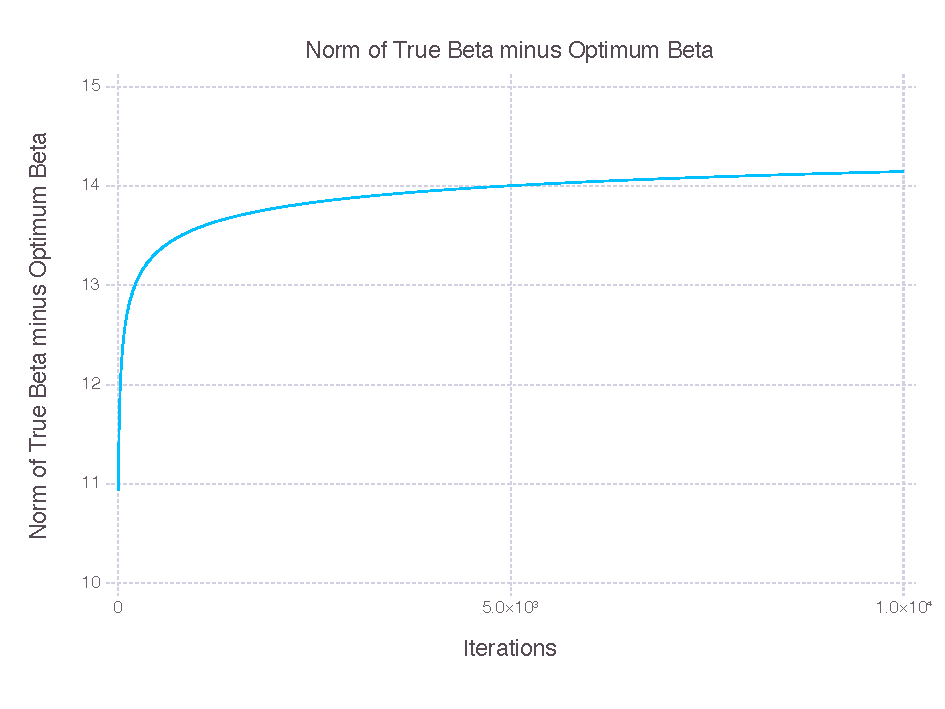
\includegraphics[width=\textwidth]{trueerrorplot4-20.pdf}
                \caption{$\lambda = 0.4$}
                \label{}
        \end{subfigure}
        \begin{subfigure}[b]{0.4\textwidth}
                \includegraphics[width=\textwidth]{{trueerrorplot5-20.pdf}}
                \caption{$\lambda = 0.5$}
                \label{}
        \end{subfigure}
        \caption{A plot of the defference between the estimate of the
          True Beta and the estimated Beta at each iteration with 20 non-sparse entries}\label{fig:trueerrors20-1}
\end{figure}
\begin{figure}
        \centering
        \begin{subfigure}[b]{0.4\textwidth}
                \includegraphics[width=\textwidth]{{trueerrorplot6-20.pdf}}
                \caption{$\lambda = 0.6$}
                \label{}
        \end{subfigure}
        \begin{subfigure}[b]{0.4\textwidth}
                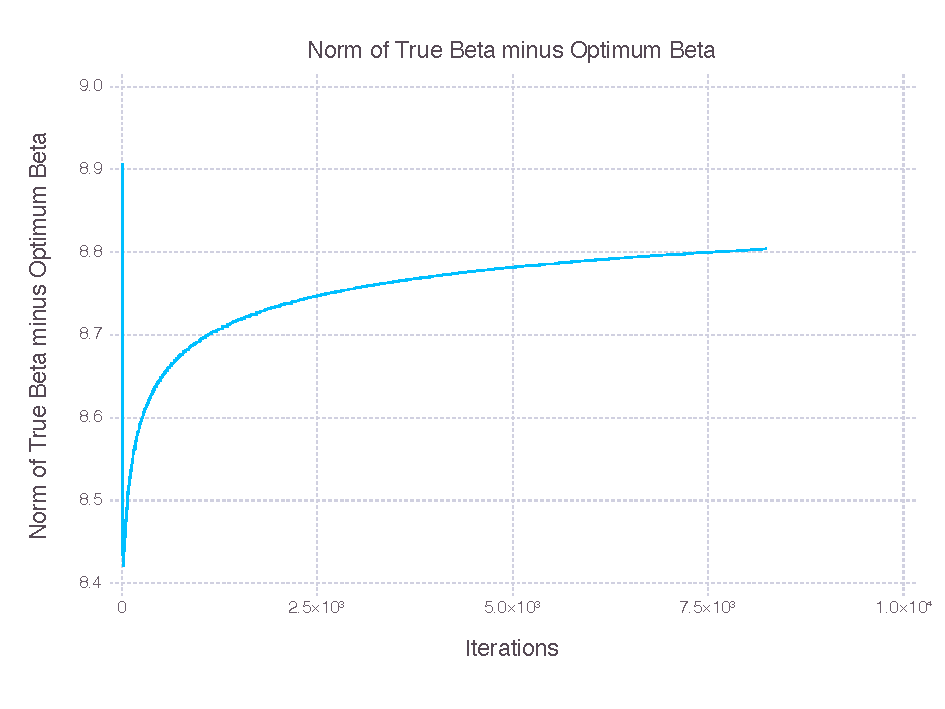
\includegraphics[width=\textwidth]{trueerrorplot7-20.pdf}
                \caption{$\lambda = 0.7$}
                \label{}
        \end{subfigure}
        \begin{subfigure}[b]{0.4\textwidth}
                \includegraphics[width=\textwidth]{{trueerrorplot8-20.pdf}}
                \caption{$\lambda = 0.8$}
                \label{}
        \end{subfigure}
        \begin{subfigure}[b]{0.4\textwidth}
                \includegraphics[width=\textwidth]{{trueerrorplot9-20.pdf}}
                \caption{$\lambda = 0.9$}
                \label{}
        \end{subfigure}
        \begin{subfigure}[b]{0.4\textwidth}
                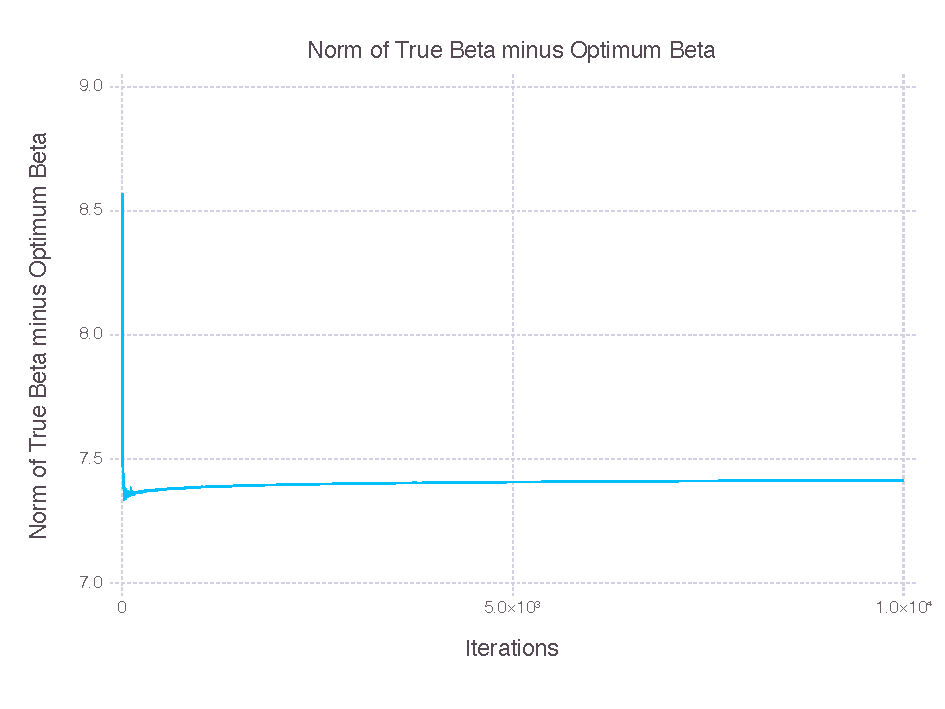
\includegraphics[width=\textwidth]{trueerrorplot10-20.pdf}
                \caption{$\lambda = 1.0$}
                \label{}
        \end{subfigure}%
        \caption{A plot of the defference between the estimate of the
          True Beta and the estimated Beta at each iteration with 20 non-sparse entries}\label{fig:trueerrors20-2}
\end{figure}
\begin{figure}
        \centering
        \begin{subfigure}[b]{0.4\textwidth}
                \includegraphics[width=\textwidth]{{trueerrorplot11-20.pdf}}
                \caption{$\lambda = 1.1$}
                \label{}
        \end{subfigure}
        \begin{subfigure}[b]{0.4\textwidth}
                \includegraphics[width=\textwidth]{{trueerrorplot12-20.pdf}}
                \caption{$\lambda = 1.2$}
                \label{}
        \end{subfigure}
        \centering
        \begin{subfigure}[b]{0.4\textwidth}
                \includegraphics[width=\textwidth]{{trueerrorplot13-20.pdf}}
                \caption{$\lambda = 1.3$}
                \label{}
        \end{subfigure}
        \begin{subfigure}[b]{0.4\textwidth}
                \includegraphics[width=\textwidth]{{trueerrorplot14-20.pdf}}
                \caption{$\lambda = 1.4$}
                \label{}
        \end{subfigure}
        \centering
        \begin{subfigure}[b]{0.4\textwidth}
                \includegraphics[width=\textwidth]{{trueerrorplot15-20.pdf}}
                \caption{$\lambda = 1.5$}
                \label{}
        \end{subfigure}
        \caption{A plot of the defference between the estimate of the
          True Beta and the estimated Beta at each iteration with 20 non-sparse entries}\label{fig:trueerrors20-3}
\end{figure}

\begin{figure}
        \centering
        \begin{subfigure}[b]{0.4\textwidth}
                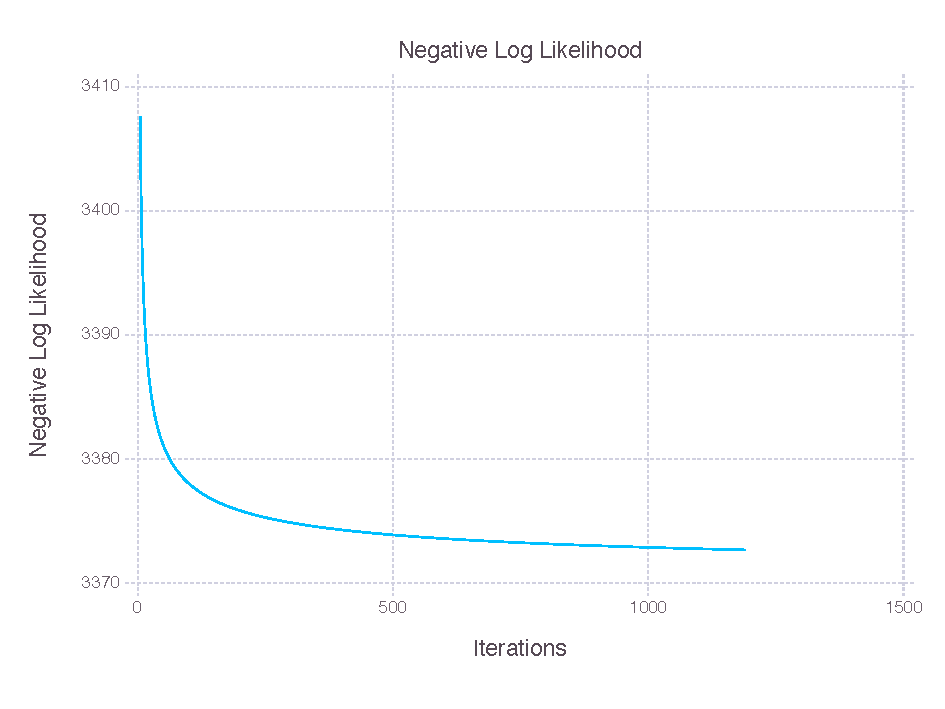
\includegraphics[width=\textwidth]{nllplot1-20.pdf}
                \caption{$\lambda = 0.1$}
                \label{}
        \end{subfigure}
        \begin{subfigure}[b]{0.4\textwidth}
                \includegraphics[width=\textwidth]{{nllplot2-20.pdf}}
                \caption{$\lambda = 0.2$}
                \label{}
        \end{subfigure}
        \begin{subfigure}[b]{0.4\textwidth}
                \includegraphics[width=\textwidth]{{nllplot3-20.pdf}}
                \caption{$\lambda = 0.3$}
                \label{}
        \end{subfigure}
        \begin{subfigure}[b]{0.4\textwidth}
                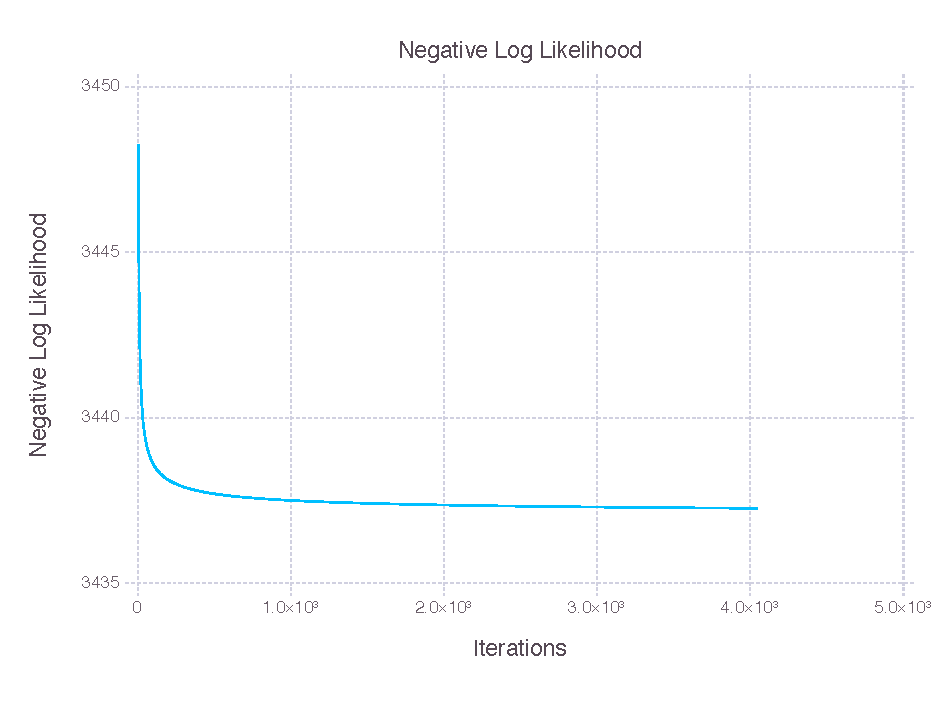
\includegraphics[width=\textwidth]{nllplot4-20.pdf}
                \caption{$\lambda = 0.4$}
                \label{}
        \end{subfigure}
        \begin{subfigure}[b]{0.4\textwidth}
                \includegraphics[width=\textwidth]{{nllplot5-20.pdf}}
                \caption{$\lambda = 0.5$}
                \label{}
        \end{subfigure}
        \caption{A plot of the errors in terms of the Negative Log
          Likelihood at each iteration with 20 non-sparse entries}\label{fig:nlls20-1}
\end{figure}
\begin{figure}
        \centering
        \begin{subfigure}[b]{0.4\textwidth}
                \includegraphics[width=\textwidth]{{nllplot6-20.pdf}}
                \caption{$\lambda = 0.6$}
                \label{}
        \end{subfigure}
        \begin{subfigure}[b]{0.4\textwidth}
                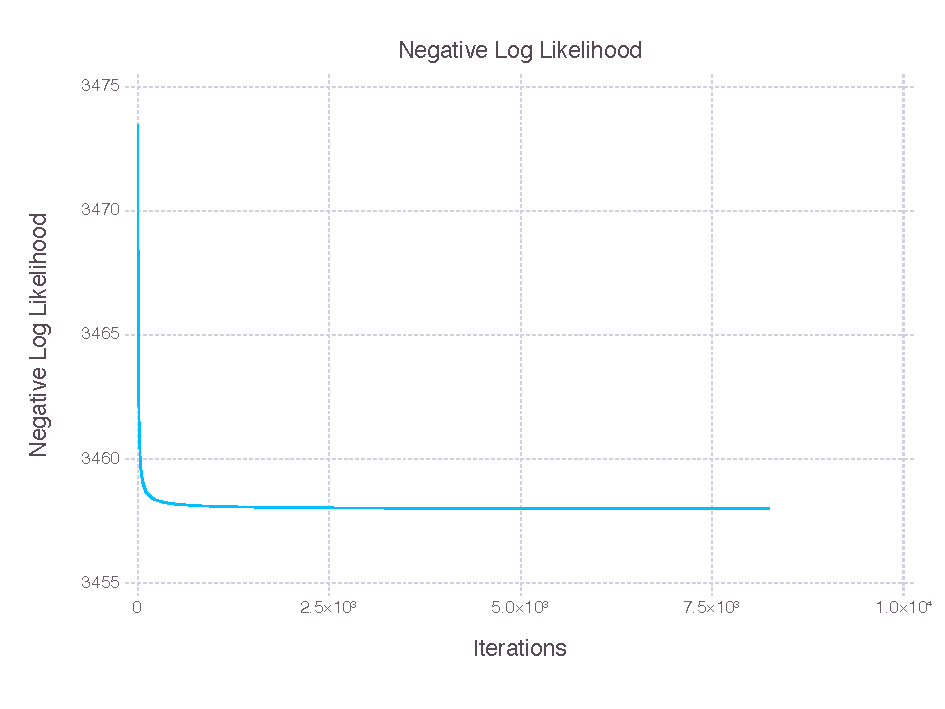
\includegraphics[width=\textwidth]{nllplot7-20.pdf}
                \caption{$\lambda = 0.7$}
                \label{}
        \end{subfigure}
        \begin{subfigure}[b]{0.4\textwidth}
                \includegraphics[width=\textwidth]{{nllplot8-20.pdf}}
                \caption{$\lambda = 0.8$}
                \label{}
        \end{subfigure}
        \begin{subfigure}[b]{0.4\textwidth}
                \includegraphics[width=\textwidth]{{nllplot9-20.pdf}}
                \caption{$\lambda = 0.9$}
                \label{}
        \end{subfigure}
        \begin{subfigure}[b]{0.4\textwidth}
                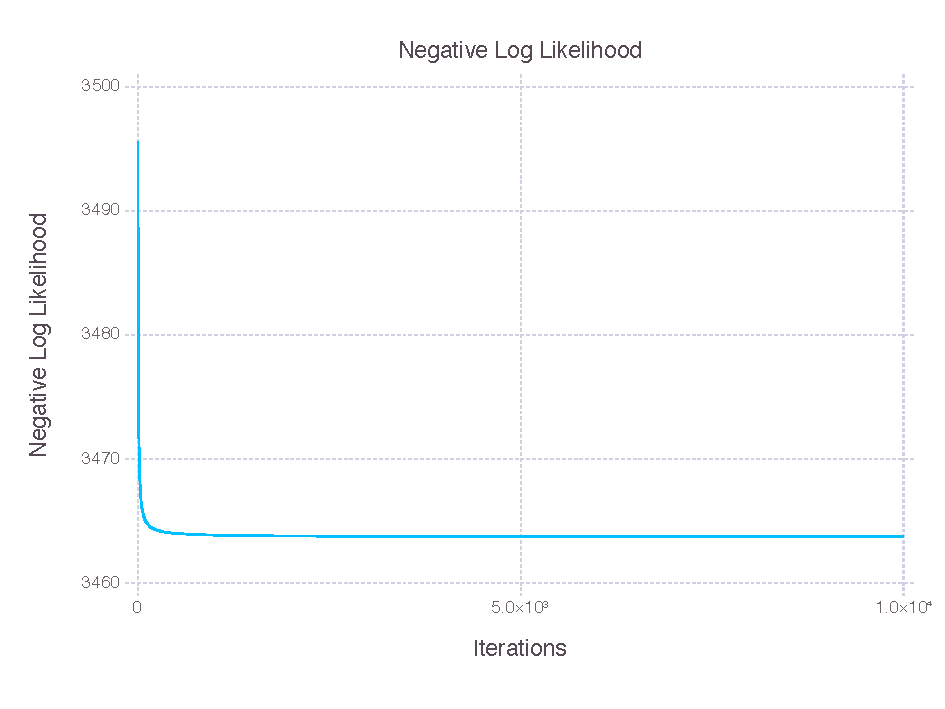
\includegraphics[width=\textwidth]{nllplot10-20.pdf}
                \caption{$\lambda = 1.0$}
                \label{}
        \end{subfigure}
        \caption{A plot of the errors in terms of the Negative Log
          Likelihood at each iteration with 20 non-sparse entries}\label{fig:nlls20-2}
\end{figure}
\begin{figure}
        \centering
        \begin{subfigure}[b]{0.4\textwidth}
                \includegraphics[width=\textwidth]{{nllplot11-20.pdf}}
                \caption{$\lambda = 1.1$}
                \label{}
        \end{subfigure}
        \begin{subfigure}[b]{0.4\textwidth}
                \includegraphics[width=\textwidth]{{nllplot12-20.pdf}}
                \caption{$\lambda = 1.2$}
                \label{}
        \end{subfigure}
        \centering
        \begin{subfigure}[b]{0.4\textwidth}
                \includegraphics[width=\textwidth]{{nllplot13-20.pdf}}
                \caption{$\lambda = 1.3$}
                \label{}
        \end{subfigure}
        \begin{subfigure}[b]{0.4\textwidth}
                \includegraphics[width=\textwidth]{{nllplot14-20.pdf}}
                \caption{$\lambda = 1.4$}
                \label{}
        \end{subfigure}
        \centering
        \begin{subfigure}[b]{0.4\textwidth}
                \includegraphics[width=\textwidth]{{nllplot15-20.pdf}}
                \caption{$\lambda = 1.5$}
                \label{}
        \end{subfigure}
        \caption{A plot of the errors in terms of the Negative Log
          Likelihood at each iteration with 20 non-sparse entries}\label{fig:nlls20-3}
\end{figure}


\begin{figure}
        \centering
        \begin{subfigure}[b]{0.4\textwidth}
                \includegraphics[width=\textwidth]{errorcplot1-75.pdf}
                \caption{$\lambda = 0.1$}
                \label{}
        \end{subfigure}
        \begin{subfigure}[b]{0.4\textwidth}
                \includegraphics[width=\textwidth]{{errorcplot2-75.pdf}}
                \caption{$\lambda = 0.2$}
                \label{}
        \end{subfigure}
        \begin{subfigure}[b]{0.4\textwidth}
                \includegraphics[width=\textwidth]{{errorcplot3-75.pdf}}
                \caption{$\lambda = 0.3$}
                \label{}
        \end{subfigure}
        \begin{subfigure}[b]{0.4\textwidth}
                \includegraphics[width=\textwidth]{errorcplot4-75.pdf}
                \caption{$\lambda = 0.4$}
                \label{}
        \end{subfigure}
        \begin{subfigure}[b]{0.4\textwidth}
                \includegraphics[width=\textwidth]{{errorcplot5-75.pdf}}
                \caption{$\lambda = 0.5$}
                \label{}
        \end{subfigure}
        \caption{A plot of the Epsilon at each
          iteration with 75 non-sparse entries}\label{fig:errorcs75-1}
\end{figure}
\begin{figure}
        \centering
        \begin{subfigure}[b]{0.4\textwidth}
                \includegraphics[width=\textwidth]{{errorcplot6-75.pdf}}
                \caption{$\lambda = 0.6$}
                \label{}
        \end{subfigure}
        \begin{subfigure}[b]{0.4\textwidth}
                \includegraphics[width=\textwidth]{errorcplot7-75.pdf}
                \caption{$\lambda = 0.7$}
                \label{}
        \end{subfigure}
        \begin{subfigure}[b]{0.4\textwidth}
                \includegraphics[width=\textwidth]{{errorcplot8-75.pdf}}
                \caption{$\lambda = 0.8$}
                \label{}
        \end{subfigure}
        \begin{subfigure}[b]{0.4\textwidth}
                \includegraphics[width=\textwidth]{{errorcplot9-75.pdf}}
                \caption{$\lambda = 0.9$}
                \label{}
        \end{subfigure}
        \begin{subfigure}[b]{0.4\textwidth}
                \includegraphics[width=\textwidth]{errorcplot10-75.pdf}
                \caption{$\lambda = 1.0$}
                \label{}
        \end{subfigure}
        \caption{A plot of the Epsilon at each
          iteration with 75 non-sparse entries}\label{fig:errorcs75-2}
\end{figure}
\begin{figure}
        \centering
        \begin{subfigure}[b]{0.4\textwidth}
                \includegraphics[width=\textwidth]{{errorcplot11-75.pdf}}
                \caption{$\lambda = 1.1$}
                \label{}
        \end{subfigure}
        \begin{subfigure}[b]{0.4\textwidth}
                \includegraphics[width=\textwidth]{{errorcplot12-75.pdf}}
                \caption{$\lambda = 1.2$}
                \label{}
        \end{subfigure}
        \centering
        \begin{subfigure}[b]{0.4\textwidth}
                \includegraphics[width=\textwidth]{{errorcplot13-75.pdf}}
                \caption{$\lambda = 1.3$}
                \label{}
        \end{subfigure}
        \begin{subfigure}[b]{0.4\textwidth}
                \includegraphics[width=\textwidth]{{errorcplot14-75.pdf}}
                \caption{$\lambda = 1.4$}
                \label{}
        \end{subfigure}
        \centering
        \begin{subfigure}[b]{0.4\textwidth}
                \includegraphics[width=\textwidth]{{errorcplot15-75.pdf}}
                \caption{$\lambda = 1.5$}
                \label{}
        \end{subfigure}
        \caption{A plot of the Epsilon at each
          iteration with 75 non-sparse entries}\label{fig:errorcs75-3}
\end{figure}


\begin{figure}
        \centering
        \begin{subfigure}[b]{0.4\textwidth}
                \includegraphics[width=\textwidth]{trueerrorplot1-75.pdf}
                \caption{$\lambda = 0.1$}
                \label{}
        \end{subfigure}
        \begin{subfigure}[b]{0.4\textwidth}
                \includegraphics[width=\textwidth]{{trueerrorplot2-75.pdf}}
                \caption{$\lambda = 0.2$}
                \label{}
        \end{subfigure}
        \begin{subfigure}[b]{0.4\textwidth}
                \includegraphics[width=\textwidth]{{trueerrorplot3-75.pdf}}
                \caption{$\lambda = 0.3$}
                \label{}
        \end{subfigure}
        \begin{subfigure}[b]{0.4\textwidth}
                \includegraphics[width=\textwidth]{trueerrorplot4-75.pdf}
                \caption{$\lambda = 0.4$}
                \label{}
        \end{subfigure}
        \begin{subfigure}[b]{0.4\textwidth}
                \includegraphics[width=\textwidth]{{trueerrorplot5-75.pdf}}
                \caption{$\lambda = 0.5$}
                \label{}
        \end{subfigure}
        \caption{A plot of the defference between the estimate of the
          True Beta and the estimated Beta at each iteration with 75 non-sparse entries}\label{fig:trueerrors}
\end{figure}
\begin{figure}
        \centering
        \begin{subfigure}[b]{0.4\textwidth}
                \includegraphics[width=\textwidth]{{trueerrorplot6-75.pdf}}
                \caption{$\lambda = 0.6$}
                \label{}
        \end{subfigure}
        \begin{subfigure}[b]{0.4\textwidth}
                \includegraphics[width=\textwidth]{trueerrorplot7-75.pdf}
                \caption{$\lambda = 0.7$}
                \label{}
        \end{subfigure}
        \begin{subfigure}[b]{0.4\textwidth}
                \includegraphics[width=\textwidth]{{trueerrorplot8-75.pdf}}
                \caption{$\lambda = 0.8$}
                \label{}
        \end{subfigure}
        \begin{subfigure}[b]{0.4\textwidth}
                \includegraphics[width=\textwidth]{{trueerrorplot9-75.pdf}}
                \caption{$\lambda = 0.9$}
                \label{}
        \end{subfigure}
        \begin{subfigure}[b]{0.4\textwidth}
                \includegraphics[width=\textwidth]{trueerrorplot10-75.pdf}
                \caption{$\lambda = 1.0$}
                \label{}
        \end{subfigure}%
        \caption{A plot of the defference between the estimate of the
          True Beta and the estimated Beta at each iteration with 75 non-sparse entries}\label{fig:trueerrors}
\end{figure}
\begin{figure}
        \centering
        \begin{subfigure}[b]{0.4\textwidth}
                \includegraphics[width=\textwidth]{{trueerrorplot11-75.pdf}}
                \caption{$\lambda = 1.1$}
                \label{}
        \end{subfigure}
        \begin{subfigure}[b]{0.4\textwidth}
                \includegraphics[width=\textwidth]{{trueerrorplot12-75.pdf}}
                \caption{$\lambda = 1.2$}
                \label{}
        \end{subfigure}
        \centering
        \begin{subfigure}[b]{0.4\textwidth}
                \includegraphics[width=\textwidth]{{trueerrorplot13-75.pdf}}
                \caption{$\lambda = 1.3$}
                \label{}
        \end{subfigure}
        \begin{subfigure}[b]{0.4\textwidth}
                \includegraphics[width=\textwidth]{{trueerrorplot14-75.pdf}}
                \caption{$\lambda = 1.4$}
                \label{}
        \end{subfigure}
        \centering
        \begin{subfigure}[b]{0.4\textwidth}
                \includegraphics[width=\textwidth]{{trueerrorplot15-75.pdf}}
                \caption{$\lambda = 1.5$}
                \label{}
        \end{subfigure}
        \caption{A plot of the defference between the estimate of the
          True Beta and the estimated Beta at each iteration with 75 non-sparse entries}\label{fig:trueerrors75-3}
\end{figure}

\begin{figure}
        \centering
        \begin{subfigure}[b]{0.4\textwidth}
                \includegraphics[width=\textwidth]{nllplot1-75.pdf}
                \caption{$\lambda = 0.1$}
                \label{}
        \end{subfigure}%
        \begin{subfigure}[b]{0.4\textwidth}
                \includegraphics[width=\textwidth]{{nllplot2-75.pdf}}
                \caption{$\lambda = 0.2$}
                \label{}
        \end{subfigure}
        \begin{subfigure}[b]{0.4\textwidth}
                \includegraphics[width=\textwidth]{{nllplot3-75.pdf}}
                \caption{$\lambda = 0.3$}
                \label{}
        \end{subfigure}
        \begin{subfigure}[b]{0.4\textwidth}
                \includegraphics[width=\textwidth]{nllplot4-75.pdf}
                \caption{$\lambda = 0.4$}
                \label{}
        \end{subfigure}
        \begin{subfigure}[b]{0.4\textwidth}
                \includegraphics[width=\textwidth]{{nllplot5-75.pdf}}
                \caption{$\lambda = 0.5$}
                \label{}
        \end{subfigure}
        \caption{A plot of the errors in terms of the Negative Log
          Likelihood at each iteration with 75 non-sparse entries}\label{fig:nlls75-1}
\end{figure}
\begin{figure}
        \centering
        \begin{subfigure}[b]{0.4\textwidth}
                \includegraphics[width=\textwidth]{{nllplot6-75.pdf}}
                \caption{$\lambda = 0.6$}
                \label{}
        \end{subfigure}
        \begin{subfigure}[b]{0.4\textwidth}
                \includegraphics[width=\textwidth]{nllplot7-75.pdf}
                \caption{$\lambda = 0.7$}
                \label{}
        \end{subfigure}
        \begin{subfigure}[b]{0.4\textwidth}
                \includegraphics[width=\textwidth]{{nllplot8-75.pdf}}
                \caption{$\lambda = 0.8$}
                \label{}
        \end{subfigure}
        \begin{subfigure}[b]{0.4\textwidth}
                \includegraphics[width=\textwidth]{{nllplot9-75.pdf}}
                \caption{$\lambda = 0.9$}
                \label{}
        \end{subfigure}
        \begin{subfigure}[b]{0.4\textwidth}
                \includegraphics[width=\textwidth]{nllplot10-75.pdf}
                \caption{$\lambda = 1.0$}
                \label{}
        \end{subfigure}%
        \caption{A plot of the errors in terms of the Negative Log
          Likelihood at each iteration with 75 non-sparse entries}\label{fig:nlls75-2}
\end{figure}
\begin{figure}
        \centering
        \begin{subfigure}[b]{0.4\textwidth}
                \includegraphics[width=\textwidth]{{nllplot11-75.pdf}}
                \caption{$\lambda = 1.1$}
                \label{}
        \end{subfigure}
        \begin{subfigure}[b]{0.4\textwidth}
                \includegraphics[width=\textwidth]{{nllplot12-75.pdf}}
                \caption{$\lambda = 1.2$}
                \label{}
        \end{subfigure}
        \centering
        \begin{subfigure}[b]{0.4\textwidth}
                \includegraphics[width=\textwidth]{{nllplot13-75.pdf}}
                \caption{$\lambda = 1.3$}
                \label{}
        \end{subfigure}
        \begin{subfigure}[b]{0.4\textwidth}
                \includegraphics[width=\textwidth]{{nllplot14-75.pdf}}
                \caption{$\lambda = 1.4$}
                \label{}
        \end{subfigure}
        \centering
        \begin{subfigure}[b]{0.4\textwidth}
                \includegraphics[width=\textwidth]{{nllplot15-75.pdf}}
                \caption{$\lambda = 1.5$}
                \label{}
        \end{subfigure}
        \caption{A plot of the errors in terms of the Negative Log
          Likelihood at each iteration with 75 non-sparse entries}\label{fig:nlls75-3}
\end{figure}

\end{document}